\begin{figure}[!htb]
\centering
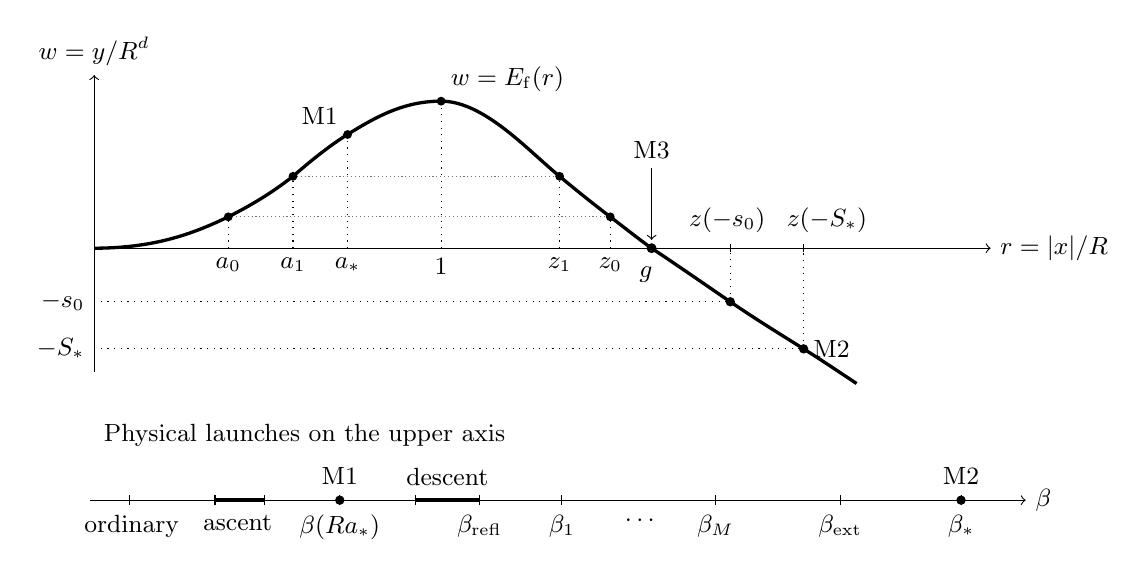
\begin{tikzpicture}[x=.99cm,y=.83cm,font=\small]
\draw[->] (0,0)--(11.5,0) node[right] {$r=|x|/R$};
\draw[->] (0,-1.9)--(0,2.65) node[above] {$w=y/R^d$};
\draw[densely dotted,black!55] (1.72,.48)--(6.62,.48)
                              (2.55,1.10)--(5.97,1.10);
\draw[very thick] (0,0) .. controls (.8,0) and (1.3,.24) .. (1.72,.48)
 .. controls (2.0,.65) and (2.26,.83) .. (2.55,1.10)
 .. controls (2.78,1.34) and (3.02,1.57) .. (3.25,1.74)
 .. controls (3.65,2.04) and (4.0,2.25) .. (4.45,2.25)
 .. controls (5.0,2.25) and (5.56,1.50) .. (5.97,1.10)
 .. controls (6.17,.90) and (6.4,.68) .. (6.62,.48)
 .. controls (6.85,.27) and (7.03,.10) .. (7.15,0)
 .. controls (7.48,-.26) and (7.89,-.60) .. (8.16,-.82)
 .. controls (8.49,-1.09) and (8.90,-1.39) .. (9.10,-1.54)
 .. controls (9.38,-1.75) and (9.60,-1.93) .. (9.78,-2.07);
\node[above right] at (4.45,2.25) {$w=E_{\rm f}(r)$};
\foreach \x/\y/\name in {1.72/.48/a_0,2.55/1.10/a_1,3.25/1.74/a_*,
                           4.45/2.25/1,5.97/1.10/z_1,6.62/.48/z_0}
  {\draw[dotted] (\x,0) node[below] {$\name$}--(\x,\y);
   \fill (\x,\y) circle (1.6pt);}
\node[above left] at (3.25,1.74) {M1};
\fill (7.15,0) circle (1.8pt) node[below=3pt,xshift=-2pt] {$g$};
\draw[->,shorten >=3pt] (7.15,1.23) node[above] {M3}--(7.15,0);
\foreach \x/\y/\level in {8.16/-.82/-s_0,9.10/-1.54/-S_*}
  {\draw[dotted] (0,\y) node[left] {$\level$}--(\x,\y)--(\x,0);
   \draw (\x,-.06)--(\x,.06);
   \fill (\x,\y) circle (1.7pt);}
\node[above=2pt] at (8.12,0) {$z(-s_0)$};
\node[above=2pt] at (9.40,0) {$z(-S_*)$};
\node[right] at (9.10,-1.54) {M2};
\begin{scope}[yshift=-3.2cm]
\node[anchor=west] at (0,1.0) {Physical launches on the upper axis};
\draw[->] (-.05,0)--(11.95,0) node[right] {$\beta$};
\foreach \x in {.45,1.55,2.18,3.15,4.12,4.94,6.00,7.97,9.57,11.12}
  \draw (\x,-.08)--(\x,.08);
\draw[line width=1.25pt] (1.55,0)--(2.18,0) (4.12,0)--(4.94,0);
\fill (3.15,0) circle (1.7pt) node[above=2pt] {M1};
\fill (11.12,0) circle (1.7pt) node[above=2pt] {M2};
\node[below] at (.48,-.08) {ordinary};
\node[below] at (1.84,-.08) {ascent};
\node[below] at (3.15,-.08) {$\beta(Ra_*)$};
\node[above] at (4.53,.08) {descent};
\node[below] at (4.94,-.08) {$\beta_{\rm refl}$};
\node[below] at (6,-.08) {$\beta_1$};
\node[below] at (7,-.08) {$\cdots$};
\node[below] at (7.97,-.08) {$\beta_M$};
\node[below] at (9.57,-.08) {$\beta_{\rm ext}$};
\node[below] at (11.12,-.08) {$\beta_*$};
\end{scope}
\end{tikzpicture}
\caption{The upper panel shows the limiting fold. The radii $a_i$ and $z_i$
lie at equal levels, $i=0,1$. M1 marks the ascending matched orbit.
M2 uses the common scaled lower intercept $-S_*$. M3 compares turns
at physical heights $0$ and $s$, both approaching $g$ in scaled
radius. The lower panel orders the actual upper launches.
The two heavy segments are the fold brackets. From $\beta_{\rm refl}$
at the plus radius $Rz_0$ to $\beta_{\rm ext}$ at scaled lower
intercept $-s_0$, the launches $\beta_i$ increase as the physical
turning heights decrease. Distances are schematic.}
\label{fig:outer-fold}
\end{figure}
